\documentclass[a4paper]{article}

\usepackage[english]{babel}
\usepackage[utf8]{inputenc}
\usepackage{amsmath}
\usepackage{amsthm}
\usepackage{amsfonts}
\usepackage{graphicx}
\usepackage{xcolor}
\usepackage{enumerate}
\usepackage[colorinlistoftodos]{todonotes}

\graphicspath{ {./images} }

\newtheorem{theorem}{Theorem}[section]
\newtheorem{corollary}{Corollary}[theorem]
\newtheorem{lemma}[theorem]{Lemma}

\title{\textsc{Superimposed Extremal Graphs}}

\author{Ray Tsai}

\date{}

\begin{document}

\maketitle
                                                                                                                                
\section{Introduction}

Given graph $G$ with $n$ vertices, let $G_1, \ldots, G_m$ be subgraphs of $G$. Let $F$ be a graph
with at least one edge. Our goal is to determine the maximum sum of the number of edges over all
$G_i$'s, i.e. $\sum_{i = 1}^m e(G_i)$, with the constraint of $E(G_i) \cap E(G_j)$ not including
some graph $F$ for all distinct $i, j$. 

\section{Content}

\begin{itemize}
  \item Examine the case where $G_1, \ldots, G_m$ are induced
  \begin{itemize}
    \item The case $F = K_3$.
    \item Color-critical $F$.
    \item Generalize to any non-bipartite $F$.
  \end{itemize}
  \item Examine the non-induced case
  \begin{itemize}
    \item The case $F = K_3$.
  \end{itemize}
\end{itemize}


\section{Induced Case}

In this section, we assume that $G_1, \ldots, G_m$ are induced subgraphs of $G$. Given graph $H$,
let $\mathcal{T}(H)$ be the graph with an additional vertex connecting to all vertices in $H$.

\subsection{Triangle Case}

\begin{theorem}
  Suppose that $E(G_i) \cap E(G_j)$ does not include $K_3$ for distinct $i, j$. Then
  \[
    \sum_{i = 1}^n e(G_i) \leq n\left\lfloor\frac{n^2}{4}\right\rfloor,
  \]
  with equality if and only if $G_1 = G_2 = \cdots = G_n = K_{\left\lceil\frac{n}{2}\right\rceil,
  \left\lfloor\frac{n}{2}\right\rfloor}$.
\end{theorem}

\begin{lemma}
  Suppose $E(G_1) \cap E(G_2)$ does not include $K_3$. Then
  \[
    e(G_1) + e(G_2) \leq 2\left\lfloor\frac{n^2}{4}\right\rfloor,
  \]
  with equality if and only if $G_1 = G_2 = K_{\left\lceil\frac{n}{2}\right\rceil,
  \left\lfloor\frac{n}{2}\right\rfloor}$, unless $n$ is odd and $G_1 = K_{\left\lceil\frac{n -
  1}{2}\right\rceil, \left\lfloor\frac{n - 1}{2}\right\rfloor}$ and $G_2 =
  \mathcal{T}(K_{\left\lceil\frac{n - 1}{2}\right\rceil, \left\lfloor\frac{n -
  1}{2}\right\rfloor})$.
\end{lemma}

\begin{proof}
  Let $C = V(G_1) \cap V(G_2)$, the set of vertices in both $G_1$ and $G_2$. Let $A = V(G_1)
  \backslash C$, and let $B = V(G_2) \backslash C$. For simplicity, put $a = |A|$, $b = |B|$, and $c
  = |C|$. We may assume that $a + b + c = n$.

  We now find an upper bound of $e(G_1) + e(G_2)$ with respect to $a, b, c$. Since $G_1, G_2$ are
  induced graphs, we have $\{u, v\} \in E(G_1)$ if and only if $\{u, v\} \in E(G_2)$, for $u, v \in
  C$. This implies the subgraph of $G_1$ induced by $C$ is identical to the subgraph of $G_2$
  induced by $C$. In other words, $E(G_1[C]) = E(G_2[C]) = E(G_i) \cap E(G_j)$, which is
  triangle-free. By Mantel's Theorem, $e(G_1[C]) \leq \left\lfloor\frac{c^2}{4}\right\rfloor$, with
  equality if and only if $G_1[C] = K_{\left\lceil\frac{c}{2}\right\rceil,
  \left\lfloor\frac{c}{2}\right\rfloor}$. Hence, we may write
  \begin{align}
    e(G_1) + e(G_2) 
    &\leq \binom{|V(G_1)|}{2} + \binom{|V(G_2)|}{2} - 2\left[\binom{c}{2} - \left\lfloor\frac{c^2}{4}\right\rfloor\right] \nonumber \\
    &= \binom{a + c}{2} + \binom{b + c}{2} - 2\left[\binom{c}{2} - \left\lfloor\frac{c^2}{4}\right\rfloor\right].
  \end{align}
  Define $f(a, b, c)$ as the function on the right-hand-side of (1). We show that $f(a, b, c)$
  attains its maximum at $a = b = 0$ and $c = n$. Note that
  \begin{align*}
    f(a, b - 2, c + 2) - f(a, b, c)
    &= \binom{a + c + 2}{2} - \binom{a + c}{2} \\
    &\qquad - 2\left[\binom{c + 2}{2} - \binom{c}{2} - \left\lfloor\frac{(c + 2)^2}{4}\right\rfloor + \left\lfloor\frac{c^2}{4}\right\rfloor\right] \\
    &= 2(a + c) + 1 - 2[2c + 1 - (c + 1)] \\
    &= 2a + 1 > 0.
  \end{align*}
  By symmetry, $f(a - 2, b, c + 2) > f(a, b, c)$, and thus $f$ attains its maximum when $c$ is $n -
  1$ or $n$, that is, $a + b \leq 1$. Equation (1) now yields, 
  \[
    e(G_1) + e(G_2) \leq f(a, b, c) \leq 2\left\lfloor\frac{n^2}{4}\right\rfloor.
  \]
  Assume that $a = 0$. When $c = n$, the equality holds only if $G_1 = G_2 =
  K_{\left\lceil\frac{n}{2}\right\rceil, \left\lfloor\frac{n}{2}\right\rfloor}$. If $c = n - 1$,
  then the equality holds only if $n$ is odd and $G_1 = G[C] = K_{\left\lceil\frac{n -
  1}{2}\right\rceil, \left\lfloor\frac{n - 1}{2}\right\rfloor}$ and $G_2$ is $G_1$ with all vertices
  connected with the only remaining vertex, that is, $G_2 = \mathcal{T}(K_{\left\lceil\frac{n -
  1}{2}\right\rceil, \left\lfloor\frac{n - 1}{2}\right\rfloor})$.
\end{proof}

We now give the proof for Theorem 3.1:

\begin{proof}[Proof of Theorem 3.1]
  We may assume that $n > 1$. Put $G_{n + i} = G_i$. By Lemma 3.2,
  \[
    \sum_{i = 1}^n e(G_i) = \frac{1}{2}\sum_{i = 1}^n (e(G_i) + e(G_{i + 1})) \leq \frac{1}{2}\sum_{i = 1}^n 2\left\lfloor\frac{n^2}{4}\right\rfloor = n\left\lfloor\frac{n^2}{4}\right\rfloor.
  \]
  Suppose the equality holds. By Lemma 3.2, we are done if $n$ is even. Suppose $n$ is odd and $G_i
   = \mathcal{T}(K_{\left\lceil\frac{n -
  1}{2}\right\rceil, \left\lfloor\frac{n - 1}{2}\right\rfloor})$ for some $i$. By Lemma 3.2, one of $G_i$ and $G_{i + 1}$ is
   $K_{\left\lceil\frac{n - 1}{2}\right\rceil, \left\lfloor\frac{n - 1}{2}\right\rfloor}$ and the
   other is $\mathcal{T}(K_{\left\lceil\frac{n -
  1}{2}\right\rceil, \left\lfloor\frac{n - 1}{2}\right\rfloor})$, for all $i$. Hence, $G_{i + 1} = K_{\left\lceil\frac{n -
   1}{2}\right\rceil, \left\lfloor\frac{n - 1}{2}\right\rfloor}, G_{i + 2} = \mathcal{T}(K_{\left\lceil\frac{n -
  1}{2}\right\rceil, \left\lfloor\frac{n - 1}{2}\right\rfloor}), \ldots$
   and the alternation proceeds. But then $G_{n + i} = G_i = K_{\left\lceil\frac{n -
   1}{2}\right\rceil, \left\lfloor\frac{n - 1}{2}\right\rfloor}$ as $n$ is odd, and this
   contradiction completes the proof.
\end{proof}

\subsection{Color-Critical Case}

We may generalize the triangle case to any color-critical $F$ in the same manner. 

\begin{theorem}
  Let $F$ be a $r$-color-critical graph with $r \geq 3$. Suppose that $E(G_i) \cap E(G_j)$ is
  $F$-free for distinct $i, j$. Then
  \[
    \sum_{i = 1}^n e(G_i) \leq n \cdot \textnormal{ex}(n, F),
  \]
  with equality if and only if $G_1 = G_2 = \cdots = G_n$ are $n$-vertex extremal graphs for $F$.
\end{theorem}

Let $T(n, r)$ denote the Turán graph of $n$ vertices and $r$ parts. Note that $T(n, r)$ is the
extremal graph for $K_r$. 

\begin{lemma}
  If $F$ is an $r$-color-critical graph, then
  \[
    \textnormal{ex}(n, F) = \textnormal{ex}(n, K_{r}).
  \]
\end{lemma}

\begin{proof}
  Since $T(n, r - 1)$ is $r - 1$ colorable, $T(n, r - 1)$ is $F$-free, and thus $\textnormal{ex}(n,
  F) \geq \textnormal{ex}(n, K_{r})$. Suppose some $F$-free graph $H$ has $\textnormal{ex}(n, K_r)$
  edges. \textcolor{red}{TODO: complete the proof.}
\end{proof}

\textcolor{red}{Is the Turan graph the only extremal graph for color critical $F$?}

\begin{lemma}
  Let $F$ be a $r$-color-critical graph with $r \geq 3$. Suppose $E(G_1) \cap E(G_2)$ does not
  include $F$. Then
  \[
    e(G_1) + e(G_2) \leq 2 \cdot \textnormal{ex}(n, F),
  \]
  with equality if and only if $G_1 = G_2$ are $n$-vertex extremal graphs for $F$, unless $r = 3$,
  $n$ is odd, $G_1$ is an $(n - 1)$-vertex extremal graph for $F$, and $G_2 = \mathcal{T}(G_1)$. 
\end{lemma}

\begin{proof}
  Let $C = V(G_1) \cap V(G_2)$, the set of vertices in both $G_1$ and $G_2$. Let $A = V(G_1)
  \backslash C$, and let $B = V(G_2) \backslash C$. For simplicity, put $a = |A|$, $b = |B|$, and $c
  = |C|$. We may assume that $a + b + c = n$. By the same argument in Lemma 3.2, $E(G_1[C]) =
  E(G_2[C]) = E(G_i) \cap E(G_j)$, which is $F$-free. Let $r = \chi(F)$. By Lemma 3.3, 
  \[
    E(G_1[C]) \leq \textnormal{ex}(n, F) = \textnormal{ex}(n, K_r),
  \]
  with equality if and only if $G_1[C]$ is the extremal graph for $F$. Hence, 
  \begin{align}
    e(G_1) + e(G_2) 
    &\leq \binom{a + c}{2} + \binom{b + c}{2} - 2\left[\binom{c}{2} - \textnormal{ex}(c, K_r)\right].
  \end{align}
  Define $f(a, b, c)$ as the function on the right-hand-side of (2). We show that $f(a, b, c)$
  attains its maximum at $a = b = 0$ and $c = n$. Note that
  \begin{align*}
    f(a, b - 2, c + 2) - f(a, b, c)
    &= \binom{a + c + 2}{2} - \binom{a + c}{2} \\
    &\;\; - 2\left[\binom{c + 2}{2} - \binom{c}{2} - \textnormal{ex}(c + 2, K_r) + \textnormal{ex}(c, K_r)\right] \\
    &= 2a - 2c - 1 + 2[\textnormal{ex}(c + 2, K_r) - \textnormal{ex}(c, K_r)].
  \end{align*}
  Since $r \geq 3$,
  \begin{align*}
    \textnormal{ex}(c + 2, K_r) - \textnormal{ex}(c, K_r) &= \textnormal{ex}(c + 2, K_r) - \textnormal{ex}(c + 1, K_r) \\
    &\qquad\qquad + \textnormal{ex}(c + 1, K_r) - \textnormal{ex}(c, K_r) \\
    &= \left(c + 2 - \left\lceil \frac{c + 2}{r - 1} \right\rceil\right) + \left(c + 1 - \left\lceil \frac{c + 1}{r - 1} \right\rceil\right) \\
    &\geq 2c + 3 - \left(\left\lceil \frac{c + 2}{2} \right\rceil + \left\lceil \frac{c + 1}{2} \right\rceil\right) = c + 1,
  \end{align*}
  so $f(a, b - 2, c + 2) - f(a, b, c) \geq 2a + 1 > 0$. By symmetry, $f(a - 2, b, c + 2) > f(a, b,
  c)$, and thus $f$ attains its maximum when $c$ is $n - 1$ or $n$, that is, $a + b \leq 1$.
  Equation (2) now yields, 
  \begin{align*}
    e(G_1) + e(G_2) \leq \max\left[2 \cdot \textnormal{ex}(n, K_r), 2 \cdot \textnormal{ex}(n - 1, K_r) + n - 1\right].
  \end{align*}
  Assume that $a = 0$. Since
  \begin{align}
    2 \cdot \textnormal{ex}(n, K_r) - [2 \cdot \textnormal{ex}(n - 1, K_r) + n - 1]
    &= 2\left(n - \left\lceil \frac{n}{r - 1} \right\rceil\right) - n + 1 \\
    &\geq n + 1 - 2\left\lceil \frac{n}{2} \right\rceil \geq 0, \nonumber
  \end{align}
  we have
  \begin{gather}
    e(G_1) + e(G_2) \leq 2 \cdot \textnormal{ex}(n, K_r).
  \end{gather}
  If $c = n$, the equality for (4) holds only if $G_1 = G_2$ are $n$-vertex extramal graphs for $F$.
  Suppose $c = n - 1$ and the equality holds. Observe that the equation (3) is equal to zero only
  when $r = 3$ and $n$ is odd. Hence, if $c = n - 1$, the equality for (4) could only be achieved
  when $r = 3$, $n$ is odd, $G_1$ is an $(n - 1)$-vertex extremal graph for $F$, and $G_2 =
  \mathcal{T}(G_1)$.
\end{proof}

Theorem 3.3 now follows from Lemma 3.5 and the same arument as in Theorem 3.1.

\subsection{Generalize to any non-bipartite $F$}

\begin{theorem}
  Let $F$ be a non-bipartite graph. Suppose that $E(G_i) \cap E(G_j)$ is $F$-free for distinct $i,
  j$. Then
  \[
    \sum_{i = 1}^n e(G_i) \leq n \cdot \textnormal{ex}(n, F),
  \]
  with equality if and only if $G_1 = G_2 = \cdots = G_n$ are $n$-vertex extremal graphs for $F$.
\end{theorem}

By the same argument as in Theorem 3.1, it suffices to prove the following lemma:

\begin{lemma}
  Let $F$ be a non-bipartite graph. Suppose $E(G_1) \cap E(G_2)$ does not include $F$. Then
  \[
    e(G_1) + e(G_2) \leq 2 \cdot \textnormal{ex}(n, F),
  \]
  with equality if and only if $G_1 = G_2$ are $n$-vertex extremal graphs for $F$, unless $n$ is
  odd, $G_1$ is an $(n - 1)$-vertex extremal graph for $F$, and $G_2 = \mathcal{T}(G_1)$. 
\end{lemma}

\begin{proof}
  Let $C = V(G_1) \cap V(G_2)$, the set of vertices in both $G_1$ and $G_2$. Let $A = V(G_1)
  \backslash C$, and let $B = V(G_2) \backslash C$. For simplicity, put $a = |A|$, $b = |B|$, $c
  = |C|$, and $r = \chi(F)$.

  We now find an upper bound of $e(G_1) + e(G_2)$ with respect to $a, b, c$. Since $G_1, G_2$ are
  induced graphs, we have $E(G_1[C]) = E(G_2[C]) = E(G[C]) = E(G_i) \cap E(G_j)$, which is $F$-free.
  Hence, we may write
  \begin{gather}
    e(G_1) + e(G_2) \leq \binom{a + c}{2} +  \binom{b + c}{2} - 2\left[\binom{c}{2} - \textnormal{ex}(c, F)\right].
  \end{gather}
  Define $f(a, b, c)$ as the function on the right-hand-side. We show that $f(a, b, c)$ attains its
  maximum at $a = b = 0$ and $c = n$. By a theorem of Simonovits, if $F$ is $r$-colorable, then
  $\text{ex}(c, F) = \text{ex}(c, K_r) + \text{ex}(c, \tilde{F})$, where $\tilde{F}$ is the family
  of residue subgraphs of $F$ after $F$ is embedded into $K_r$. Hence, we may write
  \begin{align*}
    f(a, b - 2, c + 2) - f(a, b, c)
    &= \binom{a + c + 2}{2} - \binom{a + c}{2} \\
    &\;\; - 2\left[\binom{c + 2}{2} - \binom{c}{2} - \textnormal{ex}(c + 2, F) + \textnormal{ex}(c, F)\right] \\
    &\geq 2a - 2c - 1 + 2[\textnormal{ex}(c + 2, K_r) - \textnormal{ex}(c, K_r)] > 0,
  \end{align*}
  as shown in the proof of Lemma 3.5. By symmetry, we also have $f(a - 2, b, c + 2) > f(a, b, c)$.
  Thus, $f$ attains its maximum when $c$ is $n - 1$ or $n$. Equation (5) now yields, 
  \begin{align*}
    e(G_1) + e(G_2) \leq \max\left[2 \cdot \textnormal{ex}(n, F), 2 \cdot \textnormal{ex}(n - 1, F) + n - 1\right].
  \end{align*}
  Assume that $a = 0$. Since
  \begin{align}
    2 \cdot \textnormal{ex}(n, F) - [2 \cdot \textnormal{ex}(n - 1, F) + n - 1]
    &\geq 2[\textnormal{ex}(n, K_r) - \textnormal{ex}(n - 1, K_r)] \\
    &\qquad\qquad\qquad\qquad - n + 1 \\
    &= 2\left(n - \left\lceil \frac{n}{r - 1} \right\rceil\right) - n + 1 \\
    &\geq n + 1 - 2\left\lceil \frac{n}{2} \right\rceil \geq 0, \nonumber
  \end{align}
  we have
  \begin{gather}
    e(G_1) + e(G_2) \leq 2 \cdot \textnormal{ex}(n, F).
  \end{gather}
  If $c = n$, the equality for (9) holds only if $G_1 = G_2$ are $n$-vertex extramal graphs for $F$.
  Suppose $c = n - 1$ and the equality holds. Observe that equation (6) is equal to zero only when
  $r = 3$ and $n$ is odd. Hence, if $c = n - 1$, the equality for (9) could only be achieved when $r
  = 3$, $n$ is odd, $G_1$ is an $(n - 1)$-vertex extremal graph for $F$, and $G_2 =
  \mathcal{T}(G_1)$.
\end{proof}

\section{Non-induced Case}

We now remove the assumption that $G_1, \dots, G_m$ are induced subgraphs. Again, we first consider
the triangle-free case.

\subsection{Triangle-Free Case}

\begin{theorem}
  Suppose that $E(G_i) \cap E(G_j)$ does not include $K_3$ for distinct $i, j$. Then,
  \[
    \sum_{i = 1}^m e(G_i) \leq \binom{n}{2} + (m - 1)\left\lfloor\frac{n^2}{4}\right\rfloor.
  \]
\end{theorem}

The natural extremal construction is to simply put $G_1 = K_n$ and the rest as
  $K_{\left\lceil\frac{n}{2}\right\rceil, \left\lfloor\frac{n}{2}\right\rfloor}$. However, even for
  $m = 2$ there are multiple extremal constructions. For example, put $G_1$ as
  $K_{\left\lceil\frac{n}{2}\right\rceil, \left\lfloor\frac{n}{2}\right\rfloor}$ and connect all
  possible pairs of vertices on the left part. On the other hand, put $G_2$ as
  $K_{\left\lceil\frac{n}{2}\right\rceil, \left\lfloor\frac{n}{2}\right\rfloor}$ and connect all
  possible pairs of vertices on the right part. 
  \begin{center}
    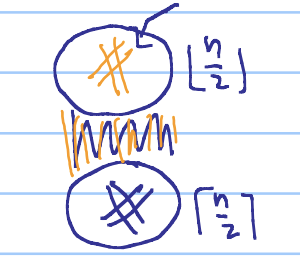
\includegraphics[width=0.3\textwidth]{non-induced-m2}
  \end{center}
  Then, $E(G_1) \cap E(G_2)$ is triangle-free and
  \begin{align*}
    e(G_1) + e(G_2) 
    &= 2e(G_1 \cap G_2) + e(G_1 \Delta G_2) \\
    &= 2\left\lfloor\frac{n^2}{4}\right\rfloor + \binom{n}{2} - \left\lfloor\frac{n^2}{4}\right\rfloor = \binom{n}{2} + \left\lfloor\frac{n^2}{4}\right\rfloor.
  \end{align*}

  Here we introduce the notation of \textit{compression} of $G_1, \ldots, G_m$, which is the graph
  obtained by moving all edges in only one $G_i$ to $G_1$. Performing compression for the case $m =
  2$, we get 
  \[
    e(G_1) + e(G_2) = e(G_1) + e(G_1 \cap G_2) \leq \binom{n}{2} + \left\lfloor\frac{n^2}{4}\right\rfloor,
  \]
  with equality if and only if $G_1 = K_n$ and $G_2 = G_1 \cap G_2 =
  K_{\left\lceil\frac{n}{2}\right\rceil, \left\lfloor\frac{n}{2}\right\rfloor}$. That is, the
  extremal graphs for $m = 2$ are isomorphic, up to compression.

  We use the notion of compression to solve for $m = 3, 4$:
  \begin{theorem}
    Suppose that $E(G_i) \cap E(G_j)$ does not include $K_3$ for distinct $i, j$. Then,
    \[
      e(G_1) + e(G_2) + e(G_3) \leq \binom{n}{2} + 2\left\lfloor\frac{n^2}{4}\right\rfloor,
    \]
    with equality if and only if $G_1 = K_n$ and $G_2, G_3 = K_{\left\lceil\frac{n}{2}\right\rceil,
    \left\lfloor\frac{n}{2}\right\rfloor}$ after compression.
  \end{theorem}

  \begin{proof}
    Compressing $G_1, G_2, G_3$ yields
    \begin{align*}
      e(G_1) + e(G_2) + e(G_3) 
      &= e(G_1) + e(G_1 \cap G_2) + e(G_1 \cap G_3) \\
      &\qquad\qquad + 2[e(G_2 \cap G_3) - e(G_1 \cap G_2 \cap G_3)] \\
      &\leq \textcolor{red}{e(G_1) + e(G_1 \cap G_2) + e(G_1 \cap G_3) \quad \text{(should be lowerbound)}} \\
      &\leq \binom{n}{2} + 2\left\lfloor\frac{n^2}{4}\right\rfloor,
    \end{align*}
    with equality if and only if $G_1 = K_n$ and $G_1 \cap G_2, G_1 \cap G_3 =
    K_{\left\lceil\frac{n}{2}\right\rceil, \left\lfloor\frac{n}{2}\right\rfloor}$. The result now
    follows.
  \end{proof}

  \textcolor{red}{TODO: solve $m = 4$.}

  % \begin{theorem}
  %   Suppose that $E(G_i) \cap E(G_j)$ does not include $K_3$ for distinct $i, j$. Then,
  %   \[
  %     \sum_{i = 1}^4 e(G_i) \leq \binom{n}{2} + 3\left\lfloor\frac{n^2}{4}\right\rfloor,
  %   \]
  %   with equality if and only if $G_1 = K_n$ and $G_i = K_{\left\lceil\frac{n}{2}\right\rceil,
  %   \left\lfloor\frac{n}{2}\right\rfloor}$ for $i > 1$ after compression.
  % \end{theorem}

  % \begin{proof}
  %   Compress $G_1, \ldots, G_m$. Put $m + 1 = 1$. By inclusion-exclusion,
  %   \begin{align*}
  %     e(G_i)
  %     &= \sum_{j \neq i} e(G_i \cap G_j) - \sum_{\substack{j, k \neq i \\ k > j}} e(G_i \cap G_j \cap G_k) + e(G_1 \cap G_2 \cap G_3 \cap G_4) \\
  %     &= \sum_{j \neq i} [e(G_i \cap G_j) - e(G_i \cap G_j)]
  %   \end{align*}
  %   for $i > 1$. Hence,
  %   \[
  %     \sum_{i = 1}^4 e(G_i) = e(G_1) + \sum_{i = 2}^{m}\sum_{k = 2}^{4} (-1)^{k}\sum_{\substack{I \subseteq [m] \\ i \in I, |I| = k}} e\left(\bigcap_{j \in I} G_j\right)
  %   \]
  % \end{proof}
\end{document}